\documentclass[10pt,oneside,a4paper,final,english]{memoir}

\usepackage{palatino}
\usepackage{microtype}
\usepackage{lscape}
\usepackage{multicol}
%\usepackage{epic,eepic}
\usepackage{latexsym}
\usepackage{verbatim}
\usepackage{listings}
\usepackage{ulem}
\usepackage{hyperref}

\let\footruleskip\undefined
\usepackage{fancyhdr}
\usepackage[final]{fixme}

\let\fref\undefined
\usepackage[plain]{fancyref}

%% FOR LOOP
\usepackage{ifthen,calc}
\newcounter{myforloopcounter}
\newcommand{\forloop}[5][1]% 
{\setcounter{#2}{#3}% 
\ifthenelse{#4}% 
{#5%
  \addtocounter{#2}{#1}% 
  \forloop[#1]{#2}{\value{#2}}{#4}{#5}% 
}%
% Else 
{}%
}% 


%% USAGE
%\forloop[step]{counter}{initial_value}{conditional}{code_block} 
\input{env/languages}
\usepackage[pdftex]{graphicx}

\DeclareGraphicsExtensions{.jpg .png .pdf}


\usepackage{amsmath}
\usepackage{latexsym}
\usepackage{amssymb}


\usepackage[osf,sc]{mathpazo}
\usepackage{microtype}
%\usepackage{fourier}
\linespread{1.05}

%\usepackage[charter]{mathdesign}
%\usepackage{lmodern}

%\usepackage{algorithmic}
%\usepackage{algorithm}

\usepackage{amsthm}


\theoremstyle{plain}  \newtheorem{definition}{Definition}
\theoremstyle{remark} \newtheorem{lemma}{Lemma}
\theoremstyle{plain}  \newtheorem{theorem}{Theorem}
\theoremstyle{remark}  \newtheorem{example}{Example}


\newcommand{\p}{\ensuremath{^\prime}}
\DeclareGraphicsExtensions{.jpg, .eps, .png}
%%% Local Variables:
%%% mode: plain-tex
%%% TeX-master: "../master"
%%% End:

\usepackage{algorithmic}
\usepackage{algorithm}
\usepackage[sectionbib,square]{natbib}
%\bibpunct{(}{)}{,}{a}{}{}
\setcitestyle{alpha}
%\setcitestyle{numbers,aysep={},yysep={;}}

\usepackage{datetime}

\chapterstyle{thatcher}

\setcounter{secnumdepth}{0}
\setcounter{tocdepth}{0}




%\pagestyle{fancy}
\begin{document}
  \fontencoding{T1}
%  \fontseries{m}
%  \fontshape{n}
%  \fontsize{12}{15}
%  \selectfont


%%%%%%%%%%%%%%%%%%%%%%%%%%%%%%%%%%%%%%%%%%%%%%%%%%%%%%%%
%                    Forside
%%%%%%%%%%%%%%%%%%%%%%%%%%%%%%%%%%%%%%%%%%%%%%%%%%%%%%%%
\makeatletter % open mode for reading @ signed variables
\def\maketitle{%
 \null
 \thispagestyle{empty}%
 \vfill
 \begin{center}\leavevmode
   \normalfont
   \LARGE{\raggedleft \@title\par}%
   \hrulefill\par
   \large{\raggedleft \subtitle\par}%
   \vskip 2cm
   {\today\par}%
 \end{center}%
 \vfill
 \begin{flushleft}
   {\large \@author } \\
   {\footnotesize \suplementInfo }
 \end{flushleft}
 \clearpage % Terminates the page here. Everything else vil be placed
            % on next page.
}
\makeatother % closing mode for reading @ signed variables
%%%%%%%%%%%%%%%%%%%%%%%%%%%%%%%%%%%%%%%%%%%%%%%%%%%%%%%%
%               Data til forside
%%%%%%%%%%%%%%%%%%%%%%%%%%%%%%%%%%%%%%%%%%%%%%%%%%%%%%%%
\title{Complementarity Problems $\cdot$ Week VI}

\def\subtitle{CCO $\cdot$ Constraint Continous Optimization}

\author{Johan Sejr Brinch Nielsen} \def\suplementInfo{

\kern 5pt \hrule width 11pc \kern 5pt

\begin{tabular}{ll}
Email: & zerrez@diku.dk  \\
Cpr.:  & 260886-2547
\end{tabular}

% putter 5pt spacing oven over og neden under stregen
\kern 5pt \hrule width 11pc \kern 5pt

Dept. of Computer Science,  \\
University of Copenhagen

}


\maketitle
\newpage

\section{Introduction}
The goal of this assignment was to implement the BFGS Quasi-Newton
method and compare this to the two methods implemented so far.

\section{Quasi-Newton Methods}
Many line search methods fall into a group, that can be identified by
a direction computation that takes the following form:
\[ p_{k+1} = - B^{-1} \nabla f(x) \]

Where $B$ is a positive definite matrix and $p_{k+1}$ is the
next search direction. This group of search methods include steepest
descent (with $B = I$) and Newton's method (with $B = \nabla f(x)$).

Quasi-Newton methods are a specific sort of line search methods that
fall into this group. They work like Newton's method, but instead of
using the Hessian, these methods approximate either this or its
inverse directly. The direction $p_k$ is hence computed as either:
\[ p_{k+1} = - B^{-1} \nabla f(x) \]
or \[ p_{k+1} = - Bi \nabla f(x) \]
Where $B$ and $Bi$ are an approximation of the Hessian and its inverse
respectively.

The new direction is now used to update the current solution by:
\[ x_{k+1} = x_k + \alpha p_{k+1} \]
Where $\alpha$ is an appropriately chosen step length.

Quasi-Newton methods may use more iterations than those, who compute
the hessian and its inverse, however each iteration costs much less in
computation time due to the approximations.

\section{Armijo Backtracking}

To figure out when a step length can be considered a good choice, some
restrictions on the resulting point has been suggested. One of these
are the Armijo condition. The Armijo condition states that the
function value in the new point should be no more than that of the
tangent of the current point (relaxed by some constant). This
condition is formalized as:
\[ f(x_k + \alpha_k p_k) \leq f(x_k) +
\alpha_k c_1 p_k^T \nabla f(x_k) \]

Where $\alpha_k$ is the current step length, $c_1$ is a constant
relaxing the condition (by raising the gradient of the limiting line)
and $p_k$ is the current search direction.

Armijo backtracking is a simple method for finding a point, that meet
the Armijo condition (hence the name). The algorithm starts with a
large step length (e.g. 1). The step length is then lowered until a
point that meets the condition is found.

If the function is descending in the chosen search direction (which is
assumed) such a point must necessarily exist. However, it may be very
close to the initial $x$. If so, the step taken can be very short,
perhaps nearly nothing at all. Therefore it is important to ensure a
minimum step size.

The algorithm can be described with the following pseudo code:
\begin{verbatim}
while not (Armijo-condition of (x+a pk)) do
  a = a * c1
end
\end{verbatim}


\section{BFGS Method}
The Broyden–Fletcher–Goldfarb–Shanno method (BFGS) is a Quasi-Newton
method. As so it approximates the inverse of the hessian. This
approximation $B_k$ is updated in each iteration like so:
\[ B_{k+1} = B_k + U_k + V_k \]

Where $U_k$ and $V_k$ are update matrices.


\section{Implementation}
This section MatLab code modified during the implementation.

\subsection*{Pseudo Code for LM}


\section{Verification}
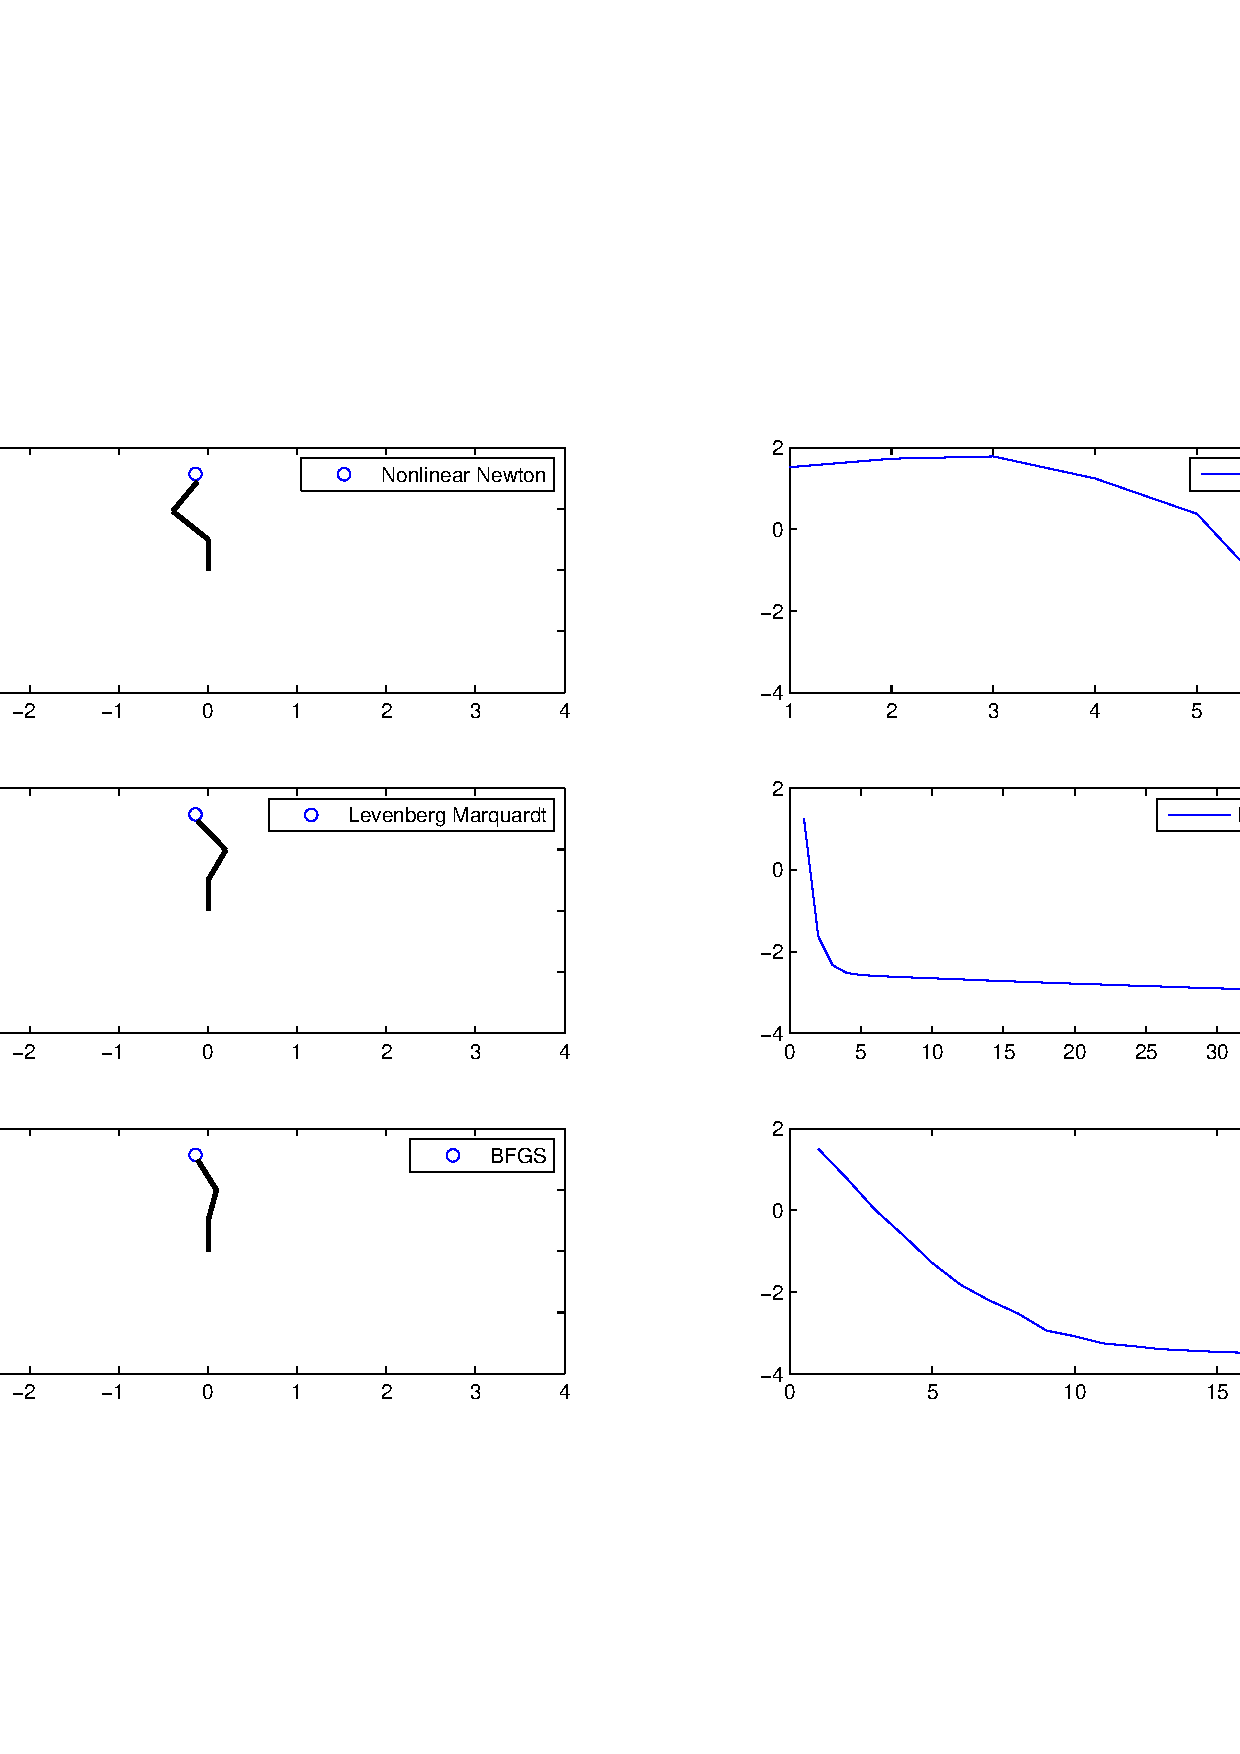
\includegraphics[width=\textwidth]{images/graph.pdf}





\end{document}

%%% Local Variables:
%%% mode: latex
%%% TeX-master: t
%%% End:
